%!TEX root = ../thesis.tex
%*******************************************************************************
%*********************************** Analysis Preservation *********
%*******************************************************************************

\chapter{Preservation and reusability}\label{ch:preservation}

\ifpdf
    \graphicspath{{chapter-preservation/Figs/Raster/}{chapter-preservation/Figs/PDF/}{chapter-preservation/Figs/}}
\else
    \graphicspath{{chapter-preservation/Figs/Vector/}{chapter-preservation/Figs/}}
\fi

Today's particle physics experiments are designed to collect physics data over a span of several decades. They operate at scales and complexities that make it impossible for the experiments to be repeated in the foreseeable future. The data taken at these experiments and physics results derived are thus extremely valuable and major problems arise from a scientific reproducibility point of view. In the following, the reusability problems directly connected to an individual analysis are discussed, and approaches taken in view of analysis preservation and analysis reinterpretation are presented. In \cref{sec:reinterpretations}, a motivation for reinterpretations is given and the necessary ingredients are described. The remaining sections discuss three efforts related to ingredients necessary \eg for large-scale reinterpretations.

\section{The case for reinterpretations}\label{sec:reinterpretations}

\subsection{Motivation}
Designing and executing searches for \gls{bsm} physics requires a substantial amount of person-power and computing resources. As laid out in detail in \cref{part:simplified_model_analysis} of this thesis, an analysis generally aims to design search regions in which a given \gls{bsm} model can be efficiently discriminated against \gls{sm} background. Although the careful design of such regions already requires significant amount of resources, it constitutes only a fraction of the work necessary for concluding the search. 
Contributions in the search regions from \gls{sm} processes need to be estimated, usually requiring expensive \gls{mc} simulation and the development of background estimation strategies. Systematic uncertainties arising from numerous sources need to be considered and estimated. 
For the \gls{bsm} signal, a similar processing pipeline involving \gls{mc} simulation, event reconstruction and event selection needs to be executed. Finally, recorded data also needs to be reconstructed and processed through the analysis-specific event selection. 
As shown in \cref{fig:pipeline_analysis}, an analysis can thus be divided into three main processing pipelines; a \textit{background pipeline}, a \textit{signal pipeline} and a \textit{data pipeline}. Only after all three processing pipelines are concluded can the next analysis step be performed---the \textit{statistical inference}, producing the final analysis results, like \eg limits on model parameters.

Due to the substantial amount of resources necessary for developing and performing an analysis, it is not feasible to develop dedicated searches for every possible \gls{bsm} scenario. Instead, analyses are typically only interpreted in a finite set of \gls{bsm} models that only have a small number of free parameters that need to be varied. Still, it is very likely that a given analysis is sensitive to a variety of different \gls{bsm} scenarios not considered in the original publication. 

Consequently, it is not surprising that there is significant interest in the \gls{hep} community to reinterpret \gls{bsm} searches in different signal models. Reinterpretations of published ATLAS searches for \gls{susy} are performed both within as well as outside of the ATLAS collaboration\improvement{some examples}. For the \gls{hep} community outside of the experimental collaborations, the results published by the analyses performed by the collaborations represent---in the context of \gls{bsm} scenarios like \gls{susy}---the only available windows into the dataset recorded. Reinterpretations of reproducible analyses are thus the only possibility to determine the implications of \gls{lhc} data for a variety of models~\cite{reinterpretation_workshop}.


Reinterpretations are however not only of interest for the wider \gls{hep} community, but also for the experimental collaborations themselves. Within ATLAS, such efforts can serve as powerful tools for shaping the future of the search program. Reinterpretations of ATLAS \gls{susy} searches in more complete \gls{susy} models like the \gls{pmssm} not only allow to state a combined sensitivity of ATLAS to more realistic \gls{susy} models, but also enable the collaboration to identify potential blind spots and parameter regions still uncovered by existing analyses. Such reinterpretations have been performed for the Run~1 dataset~\cite{pMSSM-scan-run1:2015baa,Ambrogi:2017lov}. Similar efforts, aiming to reinterpret the current ATLAS searches for \gls{susy} in the \gls{pmssm} using the full Run~2 dataset, are currently ongoing. 

 \begin{figure}
	\centering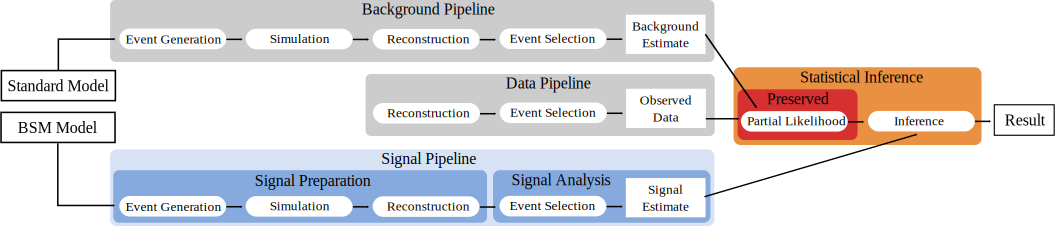
\includegraphics[width=\textwidth]{pipeline}
	\caption{Full analysis workflow including the three main processing pipelines for deriving background and signal estimates as well as observed data rates. The outputs of the three processing pipelines are combined into a likelihood forming the basis for the statistical inference. In a \textsc{Recast} setup (details in text), the background and data pipelines are archived (\eg by preserving the partial likelihood created from the background estimates and the observed data), and the signal pipeline is fully preserved, such that it can be re-executed with different inputs at any time. Figure recreated from \reference\cite{ATL-PHYS-PUB-2019-032}.}
	\label{fig:pipeline_analysis}
\end{figure}

\subsection{Approaches for reinterpretations}

As the event selection of an analysis is fixed, the pre-fit background estimates and observed data in the regions of interest targeted do not change. Hence, the data and background pipelines, shown in~\cref{fig:pipeline_analysis} and entering the statistical inference of the analysis by means of event rates, can be archived in a reusable format significantly smaller than the original input data.
In consequence, reinterpreting a search in the light of a new signal model requires the re-execution of two main analysis ingredients with (partially) new inputs; the signal pipeline and the statistical inference.

Recently, it has become technically possible to preserve the partial analysis likelihood built from the background estimates and observed data, including all auxiliary data and details of the statistical model used for inference in a pure-text format (indicated through a red box in \cref{fig:pipeline_analysis}). 
Once the signal estimates are known, a new full analysis likelihood can be built, and the viability of the new signal model can be tested with respect to the analysis in question. The publication of the full likelihood of the \onelepton search will be discussed further in~\cref{sec:full_likelihood}.

Different approaches can be taken for rendering the signal pipeline re-usable on new inputs, such that deriving signal estimates for a new \gls{bsm} scenario of interest can be derived. Manifestly the most precise approach involves running the original analysis software, but using a different \gls{bsm} model as input. As this requires the preservation of the entirety of the original software environment including the workflows used in the analysis, this is arguably the most involved approach, especially since it involves executing the computationally expensive detector simulation. 
A framework designed to facilitate such an effort, called \textsc{Recast} and originally proposed in \reference\cite{RECAST_cranmer}, is under development and aims to provide the cyber-infrastructure necessary for reinterpretations as a service. 
Through a web interface, physicists wishing to reinterpret a search with \textsc{recast}, would provide an alternative \gls{bsm} model, triggering a computational workflow re-executing the original analysis using the new signal inputs and delivering the \textit{recasted} results. \Cref{sec:recast_implementation} discusses an attempt to fully preserve the \onelepton search using the \textsc{Recast} paradigm. 

As the details of the existing \textsc{Recast} implementations of ATLAS searches for \gls{susy} are not publicly available but only meant to be interacted with through a \textsc{Recast} request, the exact implementation of the analysis selection is in general not readily available outside the ATLAS collaboration. For this reason, a number of public tools aiming to reimplement an approximated version of the event selections of a number of \gls{bsm} searches are available. Prominent examples include \textsc{CheckMate}~\cite{Checkmate2:2016npn,Checkmate:2013wra} and \textsc{MadAnalysis5}~\cite{MadAnalysis:2012fm}. ATLAS has internally maintained a similar catalogue of its \gls{susy} analyses and is publishing event selection snippets in C++ for many \gls{susy} searches on \textsc{HEPData}~\cite{HEPData:2017ypu}. Recently, this package maintained by ATLAS, called \textsc{SimpleAnalysis}~\cite{simpleanalysis}, has been made publicly available, allowing the C++ snippets published to be executed outside the collaboration.

A crucial step necessary for achieving a reliable reimplementation of the signal pipeline is the detector simulation. Executing the full detector simulation requires access to the collaborations's detector description and is computationally expensive, making it unfeasible to be used in the context of large-scale reinterpretations over a large set of models. For this reason, it is often approximated using simplified detector geometries and granularities. The most commonly used package for a fast detector simulation outside of the ATLAS collaboration is \textsc{Delphes}~\cite{Delphes:2009tx}, which is used in \eg \textsc{CheckMate} and \textsc{MadAnalysis5}. Other packages like \eg \textsc{Rivet}~\cite{Rivet1:2010ar,Rivet2:2019stt} approximate the detector response using dedicated four-vector smearing techniques, assuming that the detector response roughly factorises into the responses of single particles. Internally, ATLAS also uses a dedicated framework for four-vector smearing, used in scenarios where other fast simulation techniques are still too expensive. \Cref{sec:truth_smearing} discusses these dedicated smearing functions further.

Finally, instead of trying to estimate the signal rates of a new model using \gls{mc} simulation and (reimplemented) analysis event selections, some reinterpretation efforts like \eg \textsc{SModelS}~\cite{SModelS1:2013mwa,SModelS2:2017neo} use \textit{efficiency maps} encoding the selection and acceptance efficiencies of the analysis as a function of a subset of the analysis observables, typically the sparticle masses in the case of searches for \gls{susy}. Such efficiency maps are routinely published by the ATLAS \gls{susy} searches on \textsc{HEPData}, and allow for efficient reinterpretations as long as the signal efficiencies mostly depend on the signal kinematics and are largely independent from the specific details of the signal model~\cite{SModelS1:2013mwa}. For the \onelepton search presented herein, the efficiency maps and further analysis data products are publicly available at \reference\cite{HEPdata_1Lbb}. 

\section{Public full likelihood}\label{sec:full_likelihood}

The likelihood is arguably one of the most information-dense and valuable data products of an analysis. If the exact likelihood function of the original analysis is not known in reinterpretation efforts\footnote{Up until recently, the exact likelihood function was not part of the data products published by ATLAS searches for \gls{susy}.}, approximations need to be made for the statistical inference, \eg in terms of the correlations between event rate estimates as well as the treatment of uncertainties. Recently, in an extraordinary step towards open and reproducible science in \gls{hep}, ATLAS has started to publish full analysis likelihoods built using the \textsc{HistFactory} \gls{pdf} template~\cite{ATL-PHYS-PUB-2019-029}. This effort has been facilitated by the development of \texttt{pyhf} in conjunction with the introduction of a \texttt{JSON} specification fully describing the \textsc{HistFactory} template. As a pure-text format, the \texttt{JSON} likelihoods are human- and machine-readable, highly compressible and can easily be put under version control, all of which are properties that make them suitable for long-term preservation, which is a crucial condition for reinterpretations.

The full likelihood of the \onelepton search is publicly available at \reference\cite{fullLH_1Lbb} and is not only heavily used in the following chapters, but also in various analysis reinterpretation and combination efforts currently ongoing in ATLAS. Several efforts outside of the ATLAS collaboration have already included the analysis likelihood into their reinterpretations.
The \textsc{SModelS}~\cite{SModelS_pyhf:2020grj} and \textsc{MadAnalysis5}~\cite{Goodsell:2020ddr,Fuks:2021wpe} collaborations have both reported significant precision improvements through the use of the full likelihood. Furthermore, the full likelihood of the search presented herein has recently been used to demonstrate the concept of scalable distributed statistical inference on \glspl{hpc}~\cite{Feickert:2021sua}.
Through the \texttt{funcX} package~\cite{chard20funcx}, \texttt{pyhf} is used as a highly scalable \textit{function as a service} to fit the entire \onelepton signal grid of 125 signal points with a wall time of $\SI{156}{\second}$ using 85 available worker nodes\footnote{Theses benchmarks use \texttt{pyhf}'s \textsc{NumPy} backend and \textsc{SciPy} optimiser, a combination that has a slower log-likelihood minimisation time than \eg \textsc{PyTorch} coupled with \textsc{SciPy}, as will be shown in \cref{sec:cpu_performance}.}.

\section{Full analysis preservation using containerised workflows}\label{sec:recast_implementation}

For an analysis to be fully reusable under the \textsc{Recast} paradigm, the signal pipeline of the original analysis (cf. \cref{fig:pipeline_analysis}) needs to be preserved such that it can be re-executed on new inputs. As typically only the processing steps after the event reconstruction are analysis-specific, it is sufficient to preserve this part of the signal pipeline. Processing steps preceding the calibration and selection of physics objects only involve the central ATLAS production system and result in an ATLAS-internal data format serving as input for physics analyses. These processing steps are preserved using centrally provided ATLAS infrastructure.

 In the following, the term \textit{signal analysis} (cf.~\cref{fig:pipeline_analysis}) will refer to the analysis-specific processing steps that are not handled by the central ATLAS production system, typically starting with the selection of events that have passed the reconstruction step in~\cref{fig:pipeline_analysis}, provided in the aforementioned internal data format. Preserving the signal analysis not only needs preservation of the full software environment required for the different processing steps, but also knowledge of the correct usage of the software through parameterised job templates together with a workflow graph connecting the different processing steps. A full graph representation of the entire analysis, implemented in \textsc{Recast} is shown in \cref{fig:recast_workflow}.

\subsection{Software preservation}

As much of the software is only tested, validated and deployed on a narrow set of architectures and platforms, the full software environment defining an analysis pipeline not only includes the original analysis-specific code used for object definitions, calibrations, event selection and statistical inference, but also the operating system used and a number of low-level system libraries that the applications depend upon.
Preserving the full software environment can be achieved through the use of \textit{Docker containers}~\cite{docker,Binet:2134524} that---except for the operating system kernel---are able to package the full software environment in a portable data format, including a layered file system, the operating system as well as the actual application and all of its dependencies.
As opposed to full virtualisation, Docker containers do not rely on actual hardware virtualisation but share the operating system kernel with the host. As such, they only interact with the host through system calls to the Linux kernel~\cite{Binet:2134524}, offering a highly stable interface. This makes Docker containers a well-suited solution for deploying isolated applications on a heterogeneous computing infrastructure.

Due to the specific software structure of the \onelepton search, a containerisation requires a total of three container images spanning the following processing steps:
\begin{itemize}
	\item Event selection and physics object calibration: this step reads events in the ATLAS-internal analysis format and produces \textsc{ROOT} files with a flat structure.
	\item Determination of expected signal rates in analysis regions: the histogram-building features of \textsc{HistFitter} are exploited to generate the necessary signal histograms in the relevant selections including all systematic variations. The histograms are subsequently converted into a \textsc{JSON} patch file that can be combined with the partial, preserved likelihood to create a full analysis likelihood function.
	\item Statistical inference: although the original analysis used \textsc{HistFitter} for the statistical inference, the \textsc{Recast} implementation uses the \texttt{pyhf}-implementation of the \textsc{HistFactory} models in order to benefit from the possibility of using a partial \texttt{JSON} likelihood to preserve background and data rates. Studies have shown that the \textsc{HistFitter} and \texttt{pyhf} implementations of the statistical inference produce the same results (cf. \eg \reference\cite{ATL-PHYS-PUB-2019-029}).
\end{itemize}

The Docker images are built from suitable base images containing the software environment used for deriving the published \onelepton search results, expanded with the relevant analysis software. All docker images are subject to version control and continuous integration, such that changes to the underlying software environment can be tracked and tagged. This allows for a consistent preservation of multiple versions of the analysis pipeline. \improvement{provide dockerfiles in appendix}

\subsection{Processing steps preservation}

Preserving the software environment is not sufficient, as detailed instructions on how to use it have to be given to the user. This is achieved through parameterised job templates that specify the precise commands and arguments required to re-execute the analysis code for specific processing steps. As re-executing the analysis pipeline using different signal models involves varying input parameters, all job template parameters are exposed to the user. In \cref{fig:recast_workflow}, the parameterised job templates including their output are shown as blue rectangles, connected together through a workflow specification represented via black arrows. 

User-specifiable arguments and inputs to the event selection and physics object calibration step include the actual reconstructed \gls{mc} events in the aforementioned ATLAS-internal format, obtained through the central ATLAS production system, as well as corresponding files necessary for the pile-up correction in \gls{mc}. 
In addition, the signal process cross section as well as \gls{mc} generator-level efficiencies need to be given for the correct normalisation of the estimated signal rates to the integrated luminosity of the full Run~2 dataset. 
For each new signal model to be tested, three \gls{mc} samples need to be provided, generated with specific pile-up profiles close to the pile-up profile in data during the 2015--2016, 2017 and 2018 data-taking periods, respectively\footnote{This allows to have pile-up weights relatively close to unity, avoiding unnecessary statistical dilution.}. 
In all three jobs, the events processed are weighted according to the integrated luminosity of the data-taking period they represent within the full Run~2 dataset. A subsequent \textit{merging} step uses the same docker image as the previous processing step, and serves to merge the three produced outputs into a single \textsc{ROOT} file that can be read by the subsequent step.

Apart from the merged \textsc{ROOT} output file produced in the previous step, the generation of the expected signal rates in a \texttt{JSON} patch format requires only one additional input---a \texttt{JSON} file containing theory uncertainties on the expected signal rates. These are optional and do not have to be specified if deemed to be negligible for the signal model to be tested.

The statistical inference step requires the signal \texttt{JSON} patch from the previous step as well as the archived partial likelihood containing observed data as well as expected background rates including systematic variations thereof. 

\subsection{Workflow preservation}

Finally, the preserved processing steps need to be linked together, creating a parameterised workflow completely defining the analysis pipeline from centrally produced \gls{mc} datasets to the statistical inference results. Within \textsc{Recast}, this is achieved using the workflow description language \texttt{yadage}~\cite{yadage:2017frf}, capturing the full workflow in \texttt{YAML} format. The workflow uses the job templates and defines their processing order and dependencies.

The \textsc{Recast} implementation of the analysis presented in this work has been validated against original analysis inputs. The expected and observed CL$_s$ values derived in the original analysis were successfully re-derived using the containerised workflow implementation. On a non-isolated CPU, the full preserved analysis pipeline for a single signal model can be executed with a wall time of about $\SI{50}{\minute}$. Due to the highly portable nature of the containerised workflow, the pipeline can easily be run in a distributed setup, allowing scalable reinterpretations at full analysis precision. 


 \begin{sidewaysfigure}
	\centering\includegraphics[width=\textwidth]{yadage_workflow_instance}
	\caption{Graph of the workflow as specified for the analysis pipeline. The containerised processing steps are represented as blue rectangular nodes, while input parameters, input files and outputs are shown as red oval nodes. The workflow is comprised of four processing steps: \texttt{selection\_stage\_mc16(a,d,e)}, \texttt{merging\_stage}, \texttt{workspace\_creation\_stage} and \texttt{fitting\_stage}. The first two steps perform the object calibration, event selection and merging of the three \gls{mc} datasets representing the three data-taking periods 2015--2016, 2017 and 2018. The latter two steps implement the generation of the signal \texttt{JSON} patch as well as the final statistical inference. Compared to \cref{fig:pipeline_analysis} the first two steps implement the \textit{signal analysis} part, while the latter two steps implement the \textit{statistical inference} deriving the final results.} 
	\label{fig:recast_workflow}
\end{sidewaysfigure}


\FloatBarrier

\section{Truth-level analysis}\label{sec:truth_analysis}

\ifpdf
    \graphicspath{{chapter-pmssm/Figs/Raster/}{chapter-pmssm/Figs/PDF/}{chapter-pmssm/Figs/}}
\else
    \graphicspath{{chapter-pmssm/Figs/Vector/}{chapter-pmssm/Figs/}}
\fi

A full preservation of the entire analysis pipeline, as presented in the previous section, is highly desirable as it allows for a maximum precision reinterpretation of the original analysis using a new \gls{bsm} model. As the full detector simulation needs a significant amount of computing resources in addition to the non-negligible wall time of the actual preserved analysis pipeline, this approach can only be used on a limited set of models. In large-scale reinterpretations over high-dimensional parameter spaces, the amount of models that need to be sampled and investigated using the analysis is too high to employ the fully preserved analysis pipeline in every case. In order to significantly reduce the number of models that need to be passed through the full analysis pipeline, a pre-sorting of the models needs to be performed, filtering models for which (non-)exclusion based on a simplified analysis implementation is uncertain.

In the following, two major, complementary approaches to analysis simplifications are discussed, targeting both the \textit{signal pipeline} as well as the \textit{statistical inference} blocks in~\cref{fig:pipeline_analysis}. This section discusses the \textsc{SimpleAnalysis} implementation of the analysis, an approach implementing the signal pipeline at \textit{truth-level}, \ie using the generator-level objects without running a detector simulation. An approximation of the detector response using four-vector smearing techniques is discussed.

\Cref{ch:simplify} introduces a procedure for building simplified likelihoods from the full likelihoods of ATLAS SUSY searches in order to significantly lower the wall time needed for the statistical inference in an analysis. 
In \cref{ch:pmssm}, both approximations are combined and applied on a set of \gls{susy} models sampled from the \gls{pmssm}.

%As discussed in~\cref{ch:preservation}, the reinterpretation of an analysis involves re-executing the analysis pipeline in order to derived signal rate estimates in all regions. In large-scale reinterpretations, running a \textsc{Recast} implementation on all signal models considered is not computationally feasible and instead a \textit{truth-level} analysis is first performed for all signal models sampled. Only models with uncertain exclusion at truth-level are processed through the computationally expensive full analysis chain implemented in \textsc{Recast}. The truth-level analysis skips the detector simulation and uses generator-level objects instead. Any detector-level effects and inefficiencies will thus not be reflected in truth-level observables. In order to reproduce the kinematic distributions observed in the full analysis (using reconstruction-level objects), a dedicated \textit{truth smearing}---discussed in detail in~\cref{sec:truth_smearing}---is applied.

\subsection{Truth-level selection}\label{sec:truth_selection}

 \begin{figure}
	\centering
	\begin{subfigure}[b]{0.48\linewidth}
		\centering\includegraphics[width=\textwidth]{20210324_noLabel_noOR/700_150/lep1Pt_C1N2_Wh_hbb_700p0_150p0_smeared.pdf}
	\end{subfigure}\hfill
	\begin{subfigure}[b]{0.48\linewidth}
		\centering\includegraphics[width=\textwidth]{20210324_noLabel_noOR/700_150/jet1Pt_C1N2_Wh_hbb_700p0_150p0_smeared.pdf}
	\end{subfigure}\hfill
	\caption{Impact of the overlap removal (OR) procedure at truth-level illustrated in the lepton and leading jet transverse momenta distributions. The truth-distributions with (blue) and without (green) overlap removal (green) are compared with a reconstruction-level (orange) distribution. The exemplary benchmark signal point with $m(\charg/\neutr), m(\lsp) = 700, \SI{150}{\GeV}$ is shown in both plots. Both truth-level distributions are shown after smearing. All distributions are shown in a loose preselection requiring exactly one lepton, $\met>\SI{50}{\GeV}$, $\mt > \SI{50}{\GeV}$, and 2--3 jets, two of which need to be \textit{b}-tagged.}
	\label{fig:overlap_removal_truth}
\end{figure}

All signal and control regions considered in the original \onelepton search are implemented at truth-level using the publicly available framework \textsc{SimpleAnalysis}. The exact implementation is publicly available at \reference\cite{HEPdata_1Lbb} and was already used in~\cref{ch:uncertainties} for the derivation of some of the theory uncertainties in the full analysis.

The truth-level implementation fully specifies all object definitions introduced in~\cref{sec:object_definitions} even though some of them, like the lepton isolation, are technically not well-defined at truth-level. The four-vector smearing subsequently described is, however, in many cases implemented as a function of said object definitions and hence still allows to consider them to some extent. Additionally, as discussed in~\cref{sec:reinterpretations}, the full specification of the original analysis event selection including all object definitions allows for more straightforward reinterpretations by efforts outside of the ATLAS collaboration that generally do not have access to the original analysis software.

Following the object definitions, an overlap removal procedure following the same prescription as described for the reconstruction-level analysis is performed, \ie especially also using the same shrinking cone definitions introduced in~\cref{sec:overlap_removal}. Since tracking information is not available at truth-level, the overlap removal step removing electrons sharing a track with a muon is approximated by using a distance parameter of $\Delta R = 0.01$ between the objects. Although often neglected\footnote{The overlap removal procedures in ATLAS \gls{susy} searches tend to be quite intricate, making them non-trivial to re-implement without ATLAS and analysis-specific knowledge.} in reinterpretation efforts outside of the collaboration, the correct implementation of the overlap removal procedure employed in the original analysis is crucial to reproduce the signal estimates of the original analysis.
\Cref{fig:overlap_removal_truth} illustrates this by showing exemplary kinematic distributions of an exemplary signal point in configurations with and without overlap removal at truth-level, and comparing it with the distributions obtained at reconstruction-level\footnote{The term \textit{reconstruction-level} here refers to distributions obtained with \gls{mc} simulated datasets for which the full detector simulation and reconstruction has been run.}.
Not implementing the overlap removal procedure of the original \onelepton search results in many truth-level events not passing the analysis selections because of additional objects in the final state that would otherwise have been removed through the overlap removal. 

Finally, the exact implementation of all analysis observables is explicitly given in the \mbox{\textsc{SimpleAnalysis}} implementation, followed by the definition of all control and signal regions.

\subsection{Truth smearing}\label{sec:truth_smearing}

The general assumption of the truth smearing applied in the following is that the detector response roughly factorises into the responses of single particles. This allows to use the ATLAS detector performance results in order to construct detector response maps parameterised in different observables for each physics object. Detector response maps include object reconstruction and identification efficiencies as well as scale factors to correct for differences between \gls{mc} and observed data. Likewise, effects from the finite resolution of energy measurements in the detector are modelled through energy resolution maps. In the following, the four-vector components of electrons, muons, jets and $\etmiss$ are smeared. 
%The implementation of the smearing functions is internal to ATLAS and originates predominantly from various upgrade studies.

In the case of truth electrons, the identification efficiencies considered are parameterised in $\eta$ and $\pt$ as well as the identification working point used~\cite{PERF-2017-01}. In $\eta$, nine fixed-width bins are used. In $\pt$, six bins are implemented and a linear interpolation between two adjacent $\pt$-bins is used to get the efficiency for the given $\pt$ of each truth electron. The probability of finding a fake electron in a truth jet is estimated through a similar two-dimensional map depending on the truth jet $\eta$ and $\pt$, again using fixed-width bins in $\eta$ and a linear interpolation in $\pt$.%~\cite{PERF-2017-01}
The range of the $\pt$ interpolation for identification efficiencies and fake rates extends from $\SI{7}{\GeV}$ to $\SI{120}{\GeV}$, covering the majority of all electrons in the analysis. If the truth $\pt$ of the electron is outside of that range, the identification efficiency and fake rate from the respective bound of the corresponding $\eta$-bin are used. The probability for misidentifying an electron as a photon is estimated using different fixed values for the barrel and end-cap regions~\cite{PERF-2017-02}. Finally, the transverse energy of the electron is smeared using a random number drawn from a Gaussian distribution with  standard deviation corresponding to the $\eta$- and $\pt$-dependent energy resolution~\cite{PERF-2017-03}.

For truth muons, the identification efficiencies are also parameterised in $\eta$ and $\pt$ as well as the identification working point used~\cite{Aad:2020gmm}. Similar to truth electrons, the  $\pt$ of the muon is smeared using a Gaussian distribution with standard deviation corresponding to the momentum resolution. The momentum resolution of combined truth muons, $\sigma_\mathrm{CB}$, is computed from the measured resolutions in the \gls{id}, $\sigma_\mathrm{ID}$, and \gls{ms}, $\sigma_\mathrm{MS}$, as
\begin{equation}
	\sigma_\mathrm{CB} = \frac{\sigma_\mathrm{ID}\sigma_\mathrm{MS}}{\sqrt{\sigma_\mathrm{ID}^2 + \sigma_\mathrm{MS}^2}},
\end{equation}
where $\sigma_\mathrm{ID}$ and $\sigma_\mathrm{MS}$ are parameterised in $\eta$ and $\pt$.

The transverse momentum of truth jets is smeared using a Gaussian with standard deviation equal to the \gls{jer}, provided in a map parameterised in five bins in $\vert\eta\vert$, ranging from $\vert\eta\vert = 0$ to $\vert\eta\vert = 4.5$. The jet energy resolutions~\cite{Aad:2020flx} are provided using parameterisations of a noise $N$, stochastic $S$ and constant $C$ term for each of the seven bins in $\vert\eta\vert$, such that the resolution can be computed as
\begin{equation}
	\frac{\sigma(\pt)}{\pt} = \frac{N}{\pt}\oplus\frac{S}{\sqrt{\pt}}\oplus C.
\end{equation}
Only truth jets with $\SI{10}{\GeV} < \pt < \SI{1.5}{\TeV}$ are smeared. For truth jets with $\pt > \SI{20}{\GeV}$, the flavour tagging efficiency is considered using efficiencies parameterised in $\eta$, $\pt$ and the \textsc{MV2c10} working point (introduced in~\cref{sec:object_definitions}) used, measured in fully reconstructed simulated $\ttbar$ events~\cite{FTAG-2018-01}.

Finally, the smeared missing transverse energy is computed using the transverse momenta of all smeared truth objects in the event, including an approximation for the track soft term. The latter is approximated using resolution measurements from $Z\rightarrow \ell\ell$ events~\cite{ATLAS-CONF-2018-023}, allowing to infer a distribution of the mean soft term projected in the direction longitudinal to the total transverse momentum of all hard objects in an event, $\boldsymbol{p}_\mathrm{T}^\mathrm{hard}$. The measured resolution parallel and perpendicular to $\boldsymbol{p}_\mathrm{T}^\mathrm{hard}$ is then used to smear the nominal soft track value.
 
  \begin{figure}
	\centering
	\begin{subfigure}[b]{0.45\linewidth}
		\centering\includegraphics[width=\textwidth]{20210324/700_150/met_C1N2_Wh_hbb_700p0_150p0_smeared.pdf}
	\end{subfigure}\hfill
	\begin{subfigure}[b]{0.45\linewidth}
		\centering\includegraphics[width=\textwidth]{20210324/700_150/mt_C1N2_Wh_hbb_700p0_150p0_smeared.pdf}
	\end{subfigure}\hfill
	\begin{subfigure}[b]{0.45\linewidth}
		\centering\includegraphics[width=\textwidth]{20210324/700_150/mct_C1N2_Wh_hbb_700p0_150p0_smeared.pdf}
	\end{subfigure}\hfill
	\begin{subfigure}[b]{0.45\linewidth}
		\centering\includegraphics[width=\textwidth]{20210324/700_150/mbb_C1N2_Wh_hbb_700p0_150p0_smeared.pdf}
	\end{subfigure}\hfill
	\begin{subfigure}[b]{0.45\linewidth}
		\centering\includegraphics[width=\textwidth]{20210324/700_150/lep1Pt_C1N2_Wh_hbb_700p0_150p0_smeared.pdf}
	\end{subfigure}\hfill
	\begin{subfigure}[b]{0.45\linewidth}
		\centering\includegraphics[width=\textwidth]{20210324/700_150/jet1Pt_C1N2_Wh_hbb_700p0_150p0_smeared.pdf}
	\end{subfigure}\hfill
	\begin{subfigure}[b]{0.45\linewidth}
		\centering\includegraphics[width=\textwidth]{20210324/700_150/mlb1_C1N2_Wh_hbb_700p0_150p0_smeared.pdf}
	\end{subfigure}\hfill
	\begin{subfigure}[b]{0.45\linewidth}
		\centering\includegraphics[width=\textwidth]{20210324/700_150/nBJet30_C1N2_Wh_hbb_700p0_150p0_smeared.pdf}
	\end{subfigure}\hfill
	\caption{Comparisons of the kinematic distributions of key observables at (smeared) truth- and reconstruction-level. The exemplary benchmark signal point with $m(\charg/\neutr), m(\lsp) = 700, \SI{150}{\GeV}$ is shown. The ratio pad shows the ratio of smeared and unsmeared truth-level distributions (blue and green) to reconstruction-level distributions (orange). Only \gls{mc} statistical uncertainty is included in the error bars. All distributions are shown in a loose preselection requiring exactly one lepton, $\met>\SI{50}{\GeV}$, $\mt > \SI{50}{\GeV}$, and 2--3 jets, two of which need to be \textit{b}-tagged. The latter requirement is dropped for the \textit{b}-jet multiplicity distribution.}
	\label{fig:smearing_preselection}
\end{figure}
 
\section{Validation of the truth-level analysis}

\subsection{Validation in loose preselection}

 The performance of the truth smearing is illustrated in~\cref{fig:smearing_preselection} in a loose preselection for an exemplary benchmark signal point. The loose preselection applied requires a final state with exactly one lepton, $\met>\SI{50}{\GeV}$, $\mt > \SI{50}{\GeV}$, and 2--3 jets, two of which need to be \textit{b}-tagged. The reconstruction-level distributions are compared with the truth-level distributions before and after truth smearing. It can clearly be observed that the truth smearing noticeably improves the agreement between the truth- and reconstruction-level distributions. While the lepton and jet reconstruction and identification efficiencies are---due to their dependence on $\eta$, $\pt$ and individual working points---crucial for the overall agreement in shape, the inclusion of flavour-tagging efficiencies significantly improves the overall agreement in normalisation.
 
Although some minor differences remain, overall a good agreement is observed across all relevant kinematic distributions at loose preselection level. Most of the differences between smeared truth-level and reconstruction-level distributions in individual bins are well within the \gls{mc} statistical uncertainties arising from the relatively limited \gls{mc} statistics available.
 
 \subsection{Validation in signal regions}

 \begin{figure}
	\centering
	\begin{subfigure}[b]{0.49\linewidth}
		\centering\includegraphics[width=\textwidth]{yields_SR-LM_unsmeared}
	\end{subfigure}\hfill
	\begin{subfigure}[b]{0.49\linewidth}
		\centering\includegraphics[width=\textwidth]{yields_SR-LM_smeared}
	\end{subfigure}\hfill
	\begin{subfigure}[b]{0.49\linewidth}
		\centering\includegraphics[width=\textwidth]{yields_SR-MM_unsmeared}
	\end{subfigure}\hfill
	\begin{subfigure}[b]{0.49\linewidth}
		\centering\includegraphics[width=\textwidth]{yields_SR-MM_smeared}
	\end{subfigure}\hfill
	\begin{subfigure}[b]{0.49\linewidth}
		\centering\includegraphics[width=\textwidth]{yields_SR-HM_unsmeared}
	\end{subfigure}\hfill
	\begin{subfigure}[b]{0.49\linewidth}
		\centering\includegraphics[width=\textwidth]{yields_SR-HM_smeared}
	\end{subfigure}
	\caption{Comparison of the event rates at truth- and reconstruction-level before (left) and after (right) truth smearing. From top to bottom, the SR-LM, SR-MM and SR-HM signal regions are shown, with cumulative (integrated) $\mct$ bins. Every single point in the scatter plots represents a single signal model considered in the \onelepton search. Uncertainty bars include \gls{mc} statistical uncertainties.}
	\label{fig:smearing_signal_regions}
\end{figure}
 
 As the expected signal rates in the signal regions are ultimately what is entering the statistical inference, it is important that the good agreement observed at preselection is still present in the kinematically tighter selections of the signal regions. Additionally, it is worth investigating the agreement across all signal models considered in the original analysis, as opposed to only validating specific benchmark points. A comparison of the reconstruction-level and truth-level event rates before and after smearing in the signal regions SR-LM, SR-MM and SR-HM is shown in~\cref{fig:smearing_signal_regions} for all signal models considered in the \onelepton search. For the sake of conciseness, only the cumulative $\mct$ bins are shown in each \gls{sr} in~\cref{fig:smearing_signal_regions}. The agreement in the individual $\mct$ bins in each SR-LM, SR-MM and SR-HM is provided in~\cref{fig:smearing_signal_regions_1,fig:smearing_signal_regions_2,fig:smearing_signal_regions_3}.
 
The truth smearing drastically improves the agreement in event rate estimates at truth- and reconstruction-level across all \gls{sr} bins considered. While the event rates are generally overestimated at truth-level before smearing, compared to reconstruction-level, both tend to agree well within statistical uncertainties after smearing. 
 
\subsection{Validation using likelihood}

\begin{figure}
\floatbox[{\capbeside\thisfloatsetup{capbesideposition={right,center},capbesidewidth=0.35\textwidth}}]{figure}[\FBwidth]
{\caption{Expected and observed exclusion contours obtained with the full likelihood using reconstruction-level inputs (orange) as well as truth-level inputs before (purple) and after (green) smearing. Uncertainties include all statistical and systematic uncertainties on the background and signal for the reconstruction-level contours, but only statistical and systematic uncertainties on the background for truth-level signal inputs.}\label{fig:smearing_signal_regions}}
{\includegraphics[width=0.60\textwidth]{exclusion_1Lbb_truthInput_compareReco_BkgOnly_noLabel}}
\end{figure}

Using the nominal expected event rates at (smeared) truth-level for every signal model in the original signal grid considered in the \onelepton search, expected and observed CL$_s$ values can be computed and exclusion contours can be derived. \Cref{fig:smearing_signal_regions} compares the expected and observed exclusion contours obtained using the full likelihood and reconstruction-level signal inputs with those obtained using the full likelihood and truth-level signal inputs before and after truth smearing. While all systematic uncertainties on the signal are included in the reconstruction-level contours, no signal uncertainties are considered when obtaining both the smeared and unsmeared truth-level contours. As expected from the previous validation steps in the signal regions, the sensitivity using unsmeared truth-level signal inputs is significantly overestimated compared to the published analysis exclusion limit using reconstruction-level inputs. The smeared truth-level inputs, however, yield exclusion contours with an acceptable match compared to the reconstruction-level results.

In summary, the validation process performed at multiple selection levels of the analysis shows that the signal pipeline can be approximated reasonably well using a truth-level analysis and dedicated smearing functions. For signal models producing final states with kinematics close to those of the scenarios validated in the previous sections, this approach allows to determine the event rate estimates with high computational efficiency. In large-scale reinterpretations, the smeared truth-level analysis can be used as a basis for an efficient classification of models into two categories: models that are safely excluded or not excluded based on truth-level analysis only, and models where exclusion is in doubt and instead the precision of the full analysis pipeline using \textsc{Recast} is required.


